\documentclass[11pt]{article}
\usepackage[tmargin=0.5in,bmargin=1in,rmargin=1.5in,lmargin=1.5in]{geometry}


\usepackage{amsmath}
\usepackage{amssymb}

\usepackage{graphicx}
\usepackage{tikz}

\usepackage{ytableau}

\title{Binomial coefficients and Pascal's triangle, \\UMTYMP Advanced Topics, Fall 2020}
\date{}


\begin{document}


\maketitle

\thispagestyle{empty}

\vspace{-0.5in}

We proved the Binomial Theorem
\[ (x+y)^n = \sum_{k=0}^{n} \binom{n}{k}x^k y^{n-k}\]
where $\binom{n}{k} := \frac{n!}{k!(n-k)!}$ are the \emph{binomial coefficients}. The binomial coefficients fit into Pascal's Triangle:

\[ 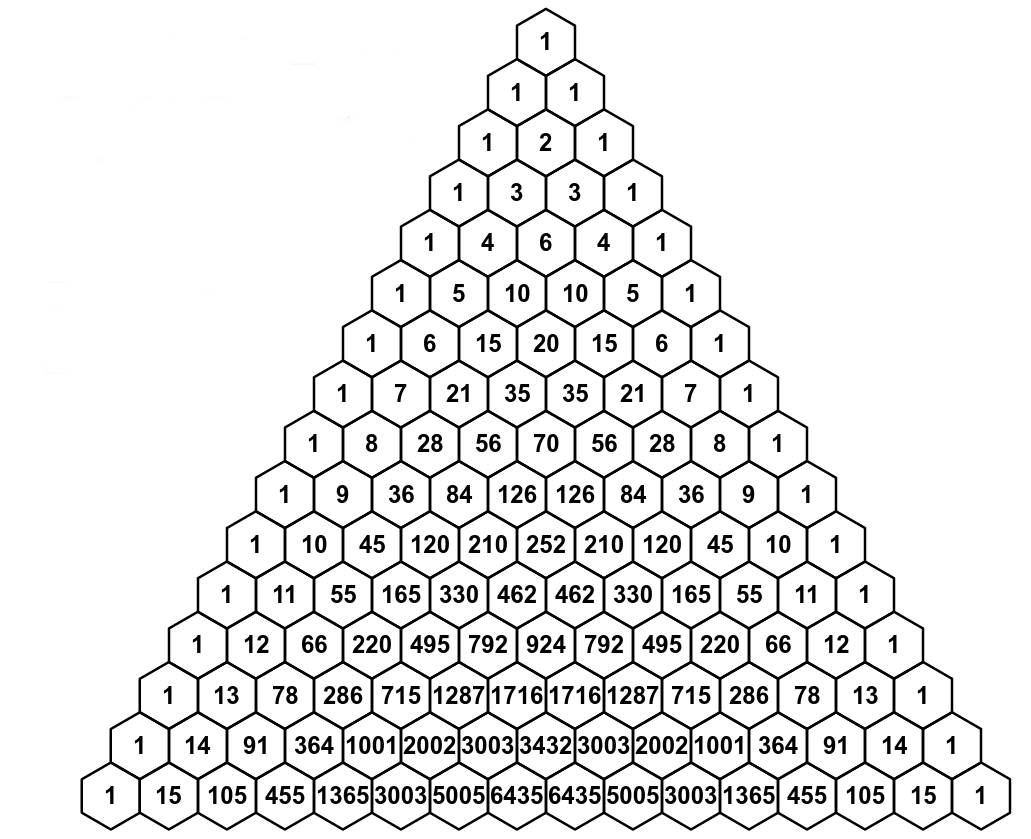
\includegraphics[width=4in]{pascal.png}\]

\medskip


\begin{enumerate}

\item Prove $\sum_{k=0}^{n} k \binom{n}{k} = n \cdot 2^{n-1}$ using the Binomial Theorem. ({\bf Hint}: derivatives!)
\item Prove $\sum_{k=0}^{n} k \binom{n}{k} = n \cdot 2^{n-1}$ combinatorially.
\item Prove $\binom{n+m}{k} = \sum_{j=0}^{k} \binom{n}{j}\binom{m}{k-j}$ combinatorially.
\item Deduce that $\sum_{k=0}^{n} \binom{n}{k}^{2} = \binom{2n}{n}$ from the previous item.
\item Prove that $\binom{k}{k} + \binom{k+1}{k} + \cdots + \binom{n}{k}=\binom{n+1}{k+1}$ combinatorially.

\medskip \medskip

\item Fill in the odd numbers in the above Pascal's triangle. Do recognize the image?

\item What about the binomial coefficients $=1 \mod 3$? (You can look up {\bf Lucas's Theorem} to learn more about arithmetic properties of binomial coefficients.)

\end{enumerate}

\end{document}
